\documentclass{zc-ust-hw}

\usepackage{lipsum}
\usepackage[]{enumitem} 
\usepackage[]{caption} 
\usepackage{subcaption}

\newcommand*{\name}{Mohammed Ali, Mohammed Khaled, SalahDin Rezk}
\newcommand*{\id}{202200594, 202200096, 202201079 }
\newcommand*{\course}{Thermodynamics, Wave Motion and Optics (PHYS201)}
\newcommand*{\assignment}{Participation 1}

\begin{document}

\maketitle

\noindent Suppose a speaker is mounted to a stand and attached to a spring having spring
constant $k = 10.0$ N/m (so it moves in a SHM). The total mass of the stand and
speaker is 2.5 kg, and the amplitude of this unit's motion is 0.500 m.

\begin{figure}[htpb]
      \begin{center}
        \hspace*{\fill}   % maximize separation between the subfigures
        \begin{subfigure}[b]{0.45\textwidth}
          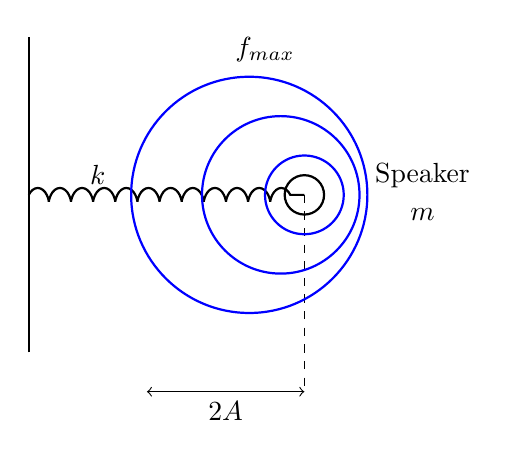
\begin{tikzpicture}[rotate=90]
            % Speaker and spring
            \draw[thick] (-2, 0) -- (2, 0);
            \draw[thick, decorate, decoration={coil, segment length=8pt}] (0, 0) -- (0, -3.5) node[near start, above] {$k$};
            \draw[thick] (0, -3.5) circle (0.25);
            \node at (0.25, -5) {Speaker};
            \node at (-0.25, -5) {$m$};

            % Dimensions
            \draw[dashed] (0, -3.5) -- (-2.5, -3.5);
            \draw[<->] (-2.5, -3.5) -- (-2.5, -1.5) node[midway, below] {$2A$};

            % Doppler effect waves
            \draw[blue, thick] (0, -3.5) circle (0.5);
            \draw[blue, thick] (0, -3.5+0.3) circle (1);
            \draw[blue, thick] (0, -3.5+0.7) circle (1.5);
            \node at (1.85, -3) {$f_{\text{max}}$};
          \end{tikzpicture}
          \caption{}%
        \end{subfigure}
        \begin{subfigure}[b]{0.45\textwidth}
          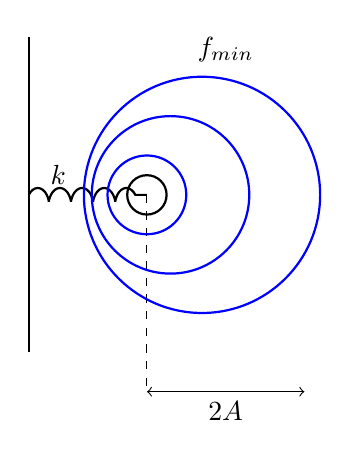
\begin{tikzpicture}[rotate=90]
            % Speaker and spring
            \draw[thick] (-2, 0) -- (2, 0);
            \draw[thick, decorate, decoration={coil, segment length=8pt}] (0, 0) -- (0, -1.5) node[near start, above] {$k$};
            \draw[thick] (0, -1.5) circle (0.25);

            % Dimensions
            \draw[dashed] (0, -1.5) -- (-2.5, -1.5);
            \draw[<->] (-2.5, -1.5) -- (-2.5, -3.5) node[midway, below] {$2A$};

            % Doppler effect waves
            \draw[blue, thick] (0, -1.5) circle (0.5);
            \draw[blue, thick] (0, -1.5-0.3) circle (1);
            \draw[blue, thick] (0, -1.5-0.7) circle (1.5);
            \node at (1.85, -2.5) {$f_{\text{min}}$};

          \end{tikzpicture}
          \caption{}%
        \end{subfigure}
      \end{center}
      \caption{}%
      \label{fig:}
    \end{figure}

\begin{enumerate}[label=(\alph*)]
  \item If the speaker emits sound waves of frequency 450 Hz, determine the
    highest and lowest frequencies heard by the person to the right of the
    speaker.

    \begin{align}
      k = 10.0 \text{ N/m}
      \quad
      m = 2.5 \text{ kg}
      \quad
      A = 0.500 \text{ m}
      \quad
      f = 450 \text{ Hz}
    .\end{align}
    \begin{align}
      f' &= f \left( \frac{v \pm v_s}{v \pm v_o} \right) \\
      f_{\text{max}} &= f \left( \frac{v + v_s}{v} \right) \\
      f_{\text{min}} &= f \left( \frac{v - v_s}{v} \right)
    .\end{align}
    % \begin{align}
    %   F = -kx \quad F = ma
    % .\end{align}
    % \begin{align}
    %   ma &= -kx \\
    %   ma + kx &= 0 \\
    %   m x'' + kx &= 0 \\
    %   x'' + \frac{k}{m} x &= 0
    % .\end{align}
    % Solution to the differential equation:
    % \begin{align}
    %     x &= A \cos\left(\omega  t\right) & \omega  = \sqrt{\frac{k}{m}} \\
    %     x' &= -A \omega \sin\left(\omega  t\right)
    % .\end{align}
    % \begin{align}
    %   v_s &= A \omega \sin\left(\omega  t\right) \\
    % .\end{align}
    \begin{align}
      v_{\text{max}} = -v_{\text{min}} &= A \sqrt{\frac{k}{m}}  \\
              &= 0.500 \sqrt{\frac{10.0}{2.5}} \\
              &= 1 \text{ m/s} \\
    .\end{align}
    \begin{align}
      f_{\text{max}} &= 450 \left( \frac{343 + 1}{343} \right) \\
                     &= 451 \text{ Hz} \\
      f_{\text{min}} &= 450 \left( \frac{343 - 1}{343} \right) \\
                     &= 449 \text{ Hz}
    .\end{align}
  \item If the maximum sound level heard by the person is 60.0 dB when he is
    closest to the speaker, 1.00 m away, what is the minimum sound level
    heard by the observer? Assume that the speed of sound is 343 m/s.
    \begin{align}
      \beta_{\text{max}} = 60.0 \text{ dB} \quad \beta=10 \log_{10}\left(\frac{I}{I_0}\right) \quad I = \frac{P}{4\pi r^2}
    .\end{align}
    \begin{align}
      \beta_{\text{max}} - \beta_{\text{min}} &= 10 \log_{10}\left(\frac{I_{\text{max}}}{I_0}\right) - 10 \log_{10}\left(\frac{I_{\text{min}}}{I_0}\right) \\
                                              &= 10 \log_{10}\left(\frac{I_{\text{max}}}{I_{\text{min}}}\right) \\
                                              &= 10 \log_{10} \left( \frac{r_{\text{min}}}{r_{\text{max}}} \right)^2 \\
                                              &= 20 \log_{10} \left( \frac{r_{\text{min}}}{r_{\text{max}}} \right) \\
                                              &= 20 \log_{10} \left( \frac{d+2A}{d} \right) \\
                                              &= 20 \log_{10} \left( \frac{1+2(0.500)}{1} \right) \\
                                              &= 6.02 \text{ dB}
    .\end{align}
    \begin{align}
      \beta_{\text{min}} &= 60.0 - 6.02 \\
                         &= 53.98 \text{ dB}
    .\end{align}
\end{enumerate}

\end{document}
